\section{Date: 2026-09-05}
\noindent \textbf{Series ID: T4244MM157NCEN} 

\noindent This series is titled Merchant Wholesalers, Except Manufacturers' Sales Branches and Offices: Nondurable Goods: Grocery and Related Products Inventories and has a frequency of Monthly, End of Month. The units are Percent and the seasonal adjustment is Not Seasonally Adjusted.The observation start date is 1992-02-01 and the observation end date is 2026-06-01.The popularity of this series is 2. \\ 

\noindent \textbf{Series ID: SESTSOCASSRGSP} 

\noindent This series is titled Real Gross Domestic Product: Social Assistance (624) in the Southeast BEA Region and has a frequency of Annual. The units are Millions of Chained 2017 Dollars and the seasonal adjustment is Not Seasonally Adjusted.The observation start date is 1997-01-01 and the observation end date is 2024-01-01.The popularity of this series is 1. \\ 

\subsection{Raw Regression}
\noindent Regresses the two series against each other directly. A significant result here can come just as easily from both series sharing a long-run trend as from any real relationship.

\begin{center}
\begin{tabular}{lclc}
\toprule
\textbf{Dep. Variable:}              & value\_fred\_SESTSOCASSRGSP & \textbf{  R-squared:         } &     0.002   \\
\textbf{Model:}                      &             OLS             & \textbf{  Adj. R-squared:    } &    -0.036   \\
\textbf{Method:}                     &        Least Squares        & \textbf{  F-statistic:       } &   0.04969   \\
\textbf{Date:}                       &       Sat, 05 Sep 2026      & \textbf{  Prob (F-statistic):} &    0.825    \\
\textbf{Time:}                       &           14:04:49          & \textbf{  Log-Likelihood:    } &   -268.33   \\
\textbf{No. Observations:}           &                28           & \textbf{  AIC:               } &     540.7   \\
\textbf{Df Residuals:}               &                26           & \textbf{  BIC:               } &     543.3   \\
\textbf{Df Model:}                   &                 1           & \textbf{                     } &             \\
\textbf{Covariance Type:}            &          nonrobust          & \textbf{                     } &             \\
\bottomrule
\end{tabular}
\begin{tabular}{lcccccc}
                                     & \textbf{coef} & \textbf{std err} & \textbf{t} & \textbf{P$> |$t$|$} & \textbf{[0.025} & \textbf{0.975]}  \\
\midrule
\textbf{const}                       &    1.963e+04  &      955.230     &    20.550  &         0.000        &     1.77e+04    &     2.16e+04     \\
\textbf{value\_fred\_T4244MM157NCEN} &     116.9651  &      524.731     &     0.223  &         0.825        &     -961.634    &     1195.564     \\
\bottomrule
\end{tabular}
\begin{tabular}{lclc}
\textbf{Omnibus:}       &  0.232 & \textbf{  Durbin-Watson:     } &    0.070  \\
\textbf{Prob(Omnibus):} &  0.891 & \textbf{  Jarque-Bera (JB):  } &    0.282  \\
\textbf{Skew:}          & -0.188 & \textbf{  Prob(JB):          } &    0.869  \\
\textbf{Kurtosis:}      &  2.684 & \textbf{  Cond. No.          } &     2.95  \\
\bottomrule
\end{tabular}
%\caption{OLS Regression Results}
\end{center}

Notes: \newline
 [1] Standard Errors assume that the covariance matrix of the errors is correctly specified.

\begin{figure}
\centering
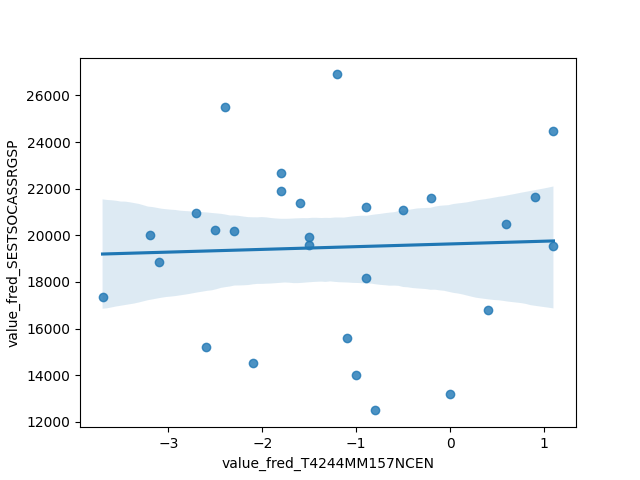
\includegraphics[scale = 0.9]{plots/plot_2026-09-05.png}
\caption{Raw Regression Plot for 2026-09-05}
\end{figure}
\newpage
\subsection{Detrended Regression}
\noindent Regresses the residuals of each series after removing its own linear time trend, so a shared trend can no longer drive the result on its own. A relationship that stays significant here is better evidence of a genuine link between the two series.

\begin{center}
\begin{tabular}{lclc}
\toprule
\textbf{Dep. Variable:}                         & value\_fred\_SESTSOCASSRGSP\_detrended & \textbf{  R-squared:         } &     0.157   \\
\textbf{Model:}                                 &                  OLS                   & \textbf{  Adj. R-squared:    } &     0.124   \\
\textbf{Method:}                                &             Least Squares              & \textbf{  F-statistic:       } &     4.824   \\
\textbf{Date:}                                  &            Sat, 05 Sep 2026            & \textbf{  Prob (F-statistic):} &   0.0372    \\
\textbf{Time:}                                  &                14:04:49                & \textbf{  Log-Likelihood:    } &   -231.94   \\
\textbf{No. Observations:}                      &                     28                 & \textbf{  AIC:               } &     467.9   \\
\textbf{Df Residuals:}                          &                     26                 & \textbf{  BIC:               } &     470.5   \\
\textbf{Df Model:}                              &                      1                 & \textbf{                     } &             \\
\textbf{Covariance Type:}                       &               nonrobust                & \textbf{                     } &             \\
\bottomrule
\end{tabular}
\begin{tabular}{lcccccc}
                                                & \textbf{coef} & \textbf{std err} & \textbf{t} & \textbf{P$> |$t$|$} & \textbf{[0.025} & \textbf{0.975]}  \\
\midrule
\textbf{const}                                  &    2.402e-11  &      187.850     &  1.28e-13  &         1.000        &     -386.131    &      386.131     \\
\textbf{value\_fred\_T4244MM157NCEN\_detrended} &    -318.6464  &      145.080     &    -2.196  &         0.037        &     -616.862    &      -20.431     \\
\bottomrule
\end{tabular}
\begin{tabular}{lclc}
\textbf{Omnibus:}       &  0.422 & \textbf{  Durbin-Watson:     } &    0.936  \\
\textbf{Prob(Omnibus):} &  0.810 & \textbf{  Jarque-Bera (JB):  } &    0.411  \\
\textbf{Skew:}          & -0.255 & \textbf{  Prob(JB):          } &    0.814  \\
\textbf{Kurtosis:}      &  2.696 & \textbf{  Cond. No.          } &     1.29  \\
\bottomrule
\end{tabular}
%\caption{OLS Regression Results}
\end{center}

Notes: \newline
 [1] Standard Errors assume that the covariance matrix of the errors is correctly specified.

\begin{figure}
\centering
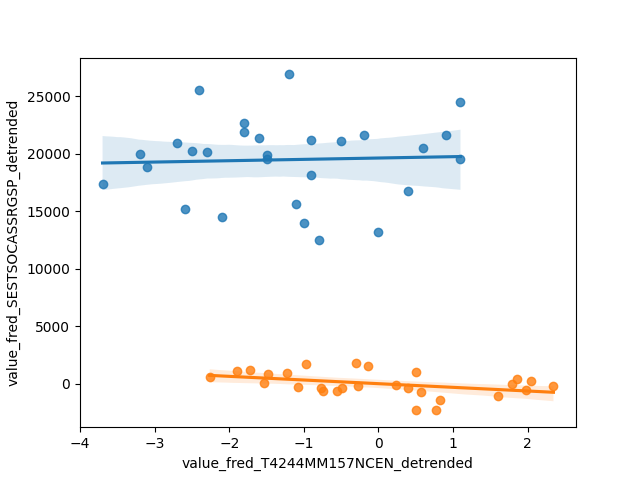
\includegraphics[scale = 0.9]{plots/plot_2026-09-05_detrended.png}
\caption{Detrended Regression Plot for 2026-09-05}
\end{figure}
\newpage
